\documentclass[a4paper,12pt]{article}
\usepackage{a4wide}
\usepackage{acronym}
\usepackage{graphicx}
\usepackage[title,titletoc,toc]{appendix}


\begin{document}

\begin{center}
{\LARGE\bf Travelling Thief Problem}\\
\vspace{0.5cm}
{\Large\bf Evolutionary Computation}\\
\vspace{1cm}
Prepared by William Reid, Matthew Hart, Samantha Peachey \& Alec Bellati\\
\vspace{1cm}
School of Computer Science,\\
The University of Adelaide\\
\vspace{1cm}
\today
\end{center}



\section*{Exercise 4}
In the planning phase, two algorithms were conceptualised that could potentially solve the Travelling Thief Problem. The first of these algorithms was based on the ``Ant Colony Optimisation'' method that was discussed in lectures. The second was an optimisation to the naive solution based on a recognised heuristic of the problem that taking items early in the tour is likely to be more expensive than taking items as late in the tour as possible.

\subsection*{Algorithm 2: Late Item Collection}
\begin{figure}[h]
\centering
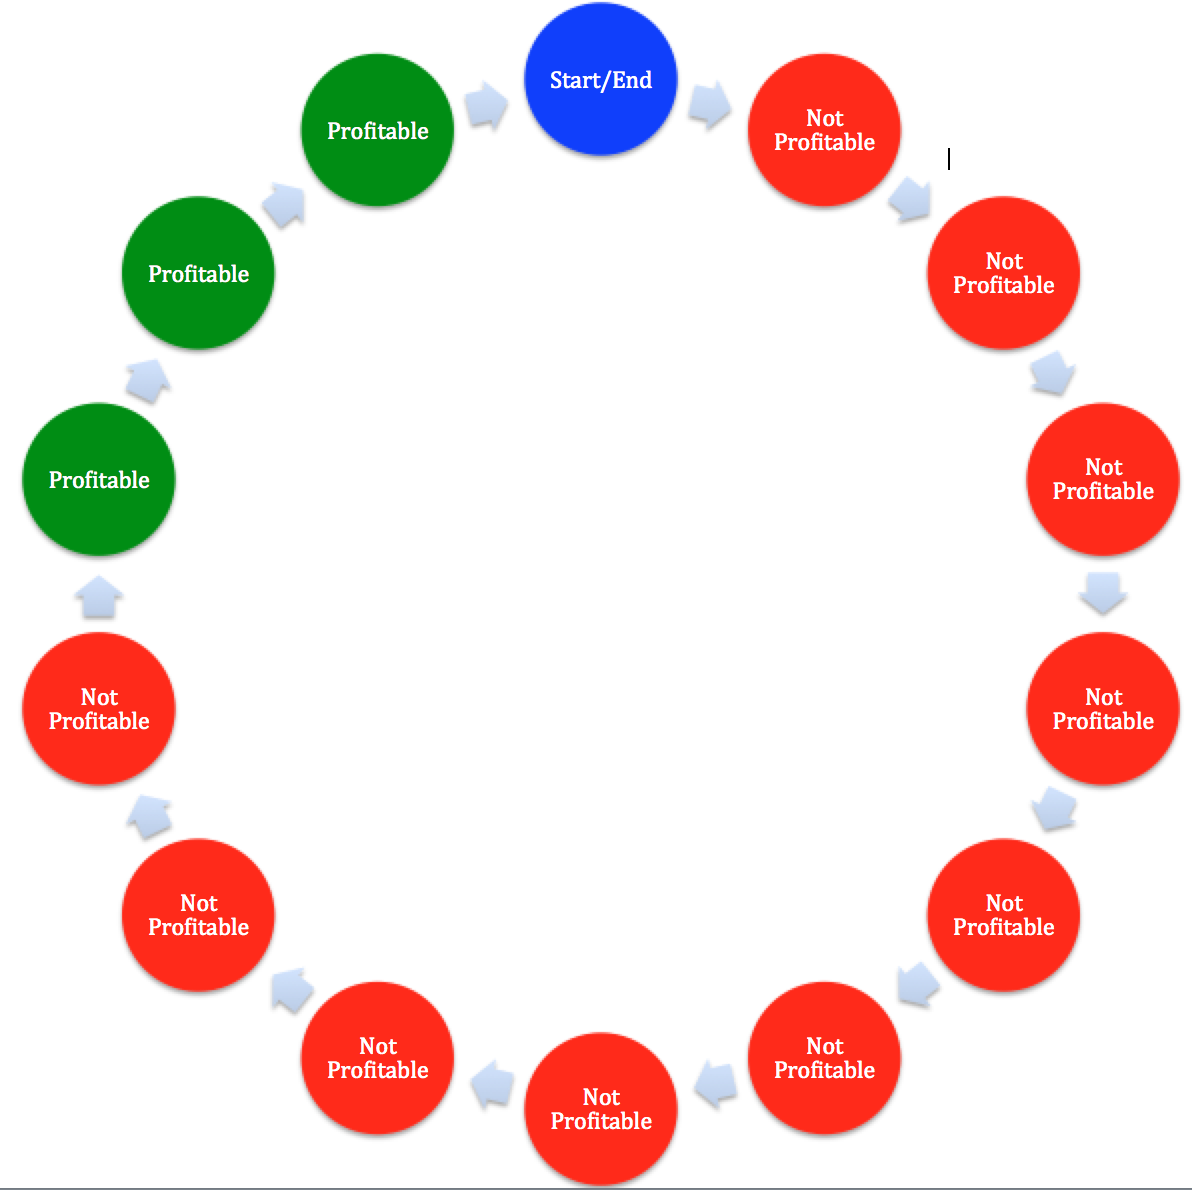
\includegraphics[width=80mm]{AlgorithmIdea.png}
\end{figure}
The Late Item Collection algorithm came to light by the acknowledgement of the following heuristic:

\begin{center}
\emph{Items taken at the start of a tour will cost the thief more money to transport than items taken later in the tour.}
\end{center}

This acknowledgement lead to the idea that if we were to rank each item by its profitability and organise the tour such that the most profitable items were taken as late in the tour as possible, this should lead to a reasonable solution to the Travelling Thief Problem.\\
The implementation of this algorithm was broken down into 5 parts:

\subsubsection*{1. Rank Each Item}
Every item in every city is given a ranking. This ranking is based on the profit of the item versus the weight of the item.
\begin{center}
\emph{profitOfItem/weightOfItem}
\end{center}

\subsubsection*{2. Fill Knapsack}
\begin{figure}[h]
\centering
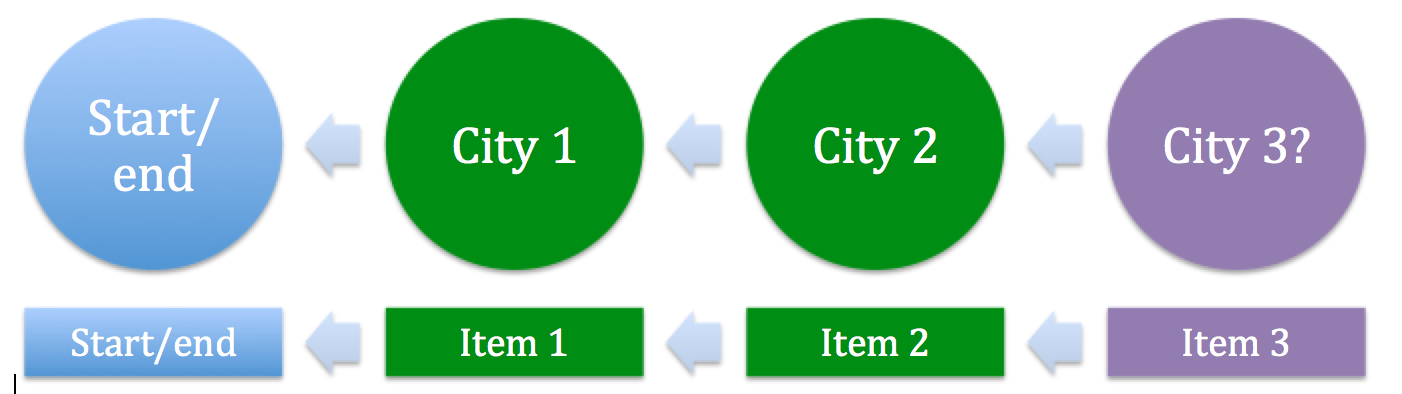
\includegraphics[width=80mm]{AddItem.png}
\end{figure}
Based on this ranking each item (in order of its rank) was tested to see if it was profitable. This was done by selecting each item (from highest ranked to lowest ranked) and then recreating the tour backwards to see if the item was profitable. For example, if an item in city 1 and 2 have already been decided to be profitable, then an item in city 3 would be tested to see if this item increases the overall profit by adding its profit and weight to the end of the chain and then evaluating the profit of this addition.

\subsubsection*{3. Split profitable/non-profitable Cities}
Based on the items taken in step two, the set of cities is now split into two subsets:

\begin{enumerate}
\item The set of non-profitable cities (visualised in red in figure 1)
\item The set of profitable cities (visualised in green in figure 1)
\end{enumerate}

\subsubsection*{3. Non-Profitable Cities}
For the set of non-profitable cities, this now becomes a simple TSP problem which is passed to our TSP solver created in assignment 1 to minimise distance travelled by the Thief (thus minimising losses).

\subsubsection*{4. Profitable Cities}
The set of profitable cities are currently ordered by the Item rank. However, this may not be the optimal tour for these cities because different permutations of this subset may yield a higher profit. For this reason I created a new selector that determined the best individual within a population based on the maximum profit. To do this I essentially reimplemented evaluate such that it would work on a subset of the problem, instead of only working on the problem space as a whole (getBestTTPSolution can be found in Population.java).

\subsubsection*{5. Recombine the subsets}
Finally, the two subsets need to be combined into the final solution. This is done by taking the best individual from step 3 and prefixing this to the best individual from step 4. Once the two subsets have been recombined into a final solution, this is then sent to TTPSolution and TTPInstance.evaluate to obtain the objective function.


\subsection*{Results}
Unfortunately, the Late Item Collection algorithm does not perform very well, getting poor results on small, medium and large datasets - splitting the problem space into two subsets, whilst a good heuristic, allows for bad results.

Upon analysis, the reason for this is that splitting the problem into two subsets allows for a potentially good solution within the subsets themselves, but when recombined, the solution allows for expensive edge costs within the tour as a whole (as displayed in figure 3).
\begin{figure}[h]
\centering
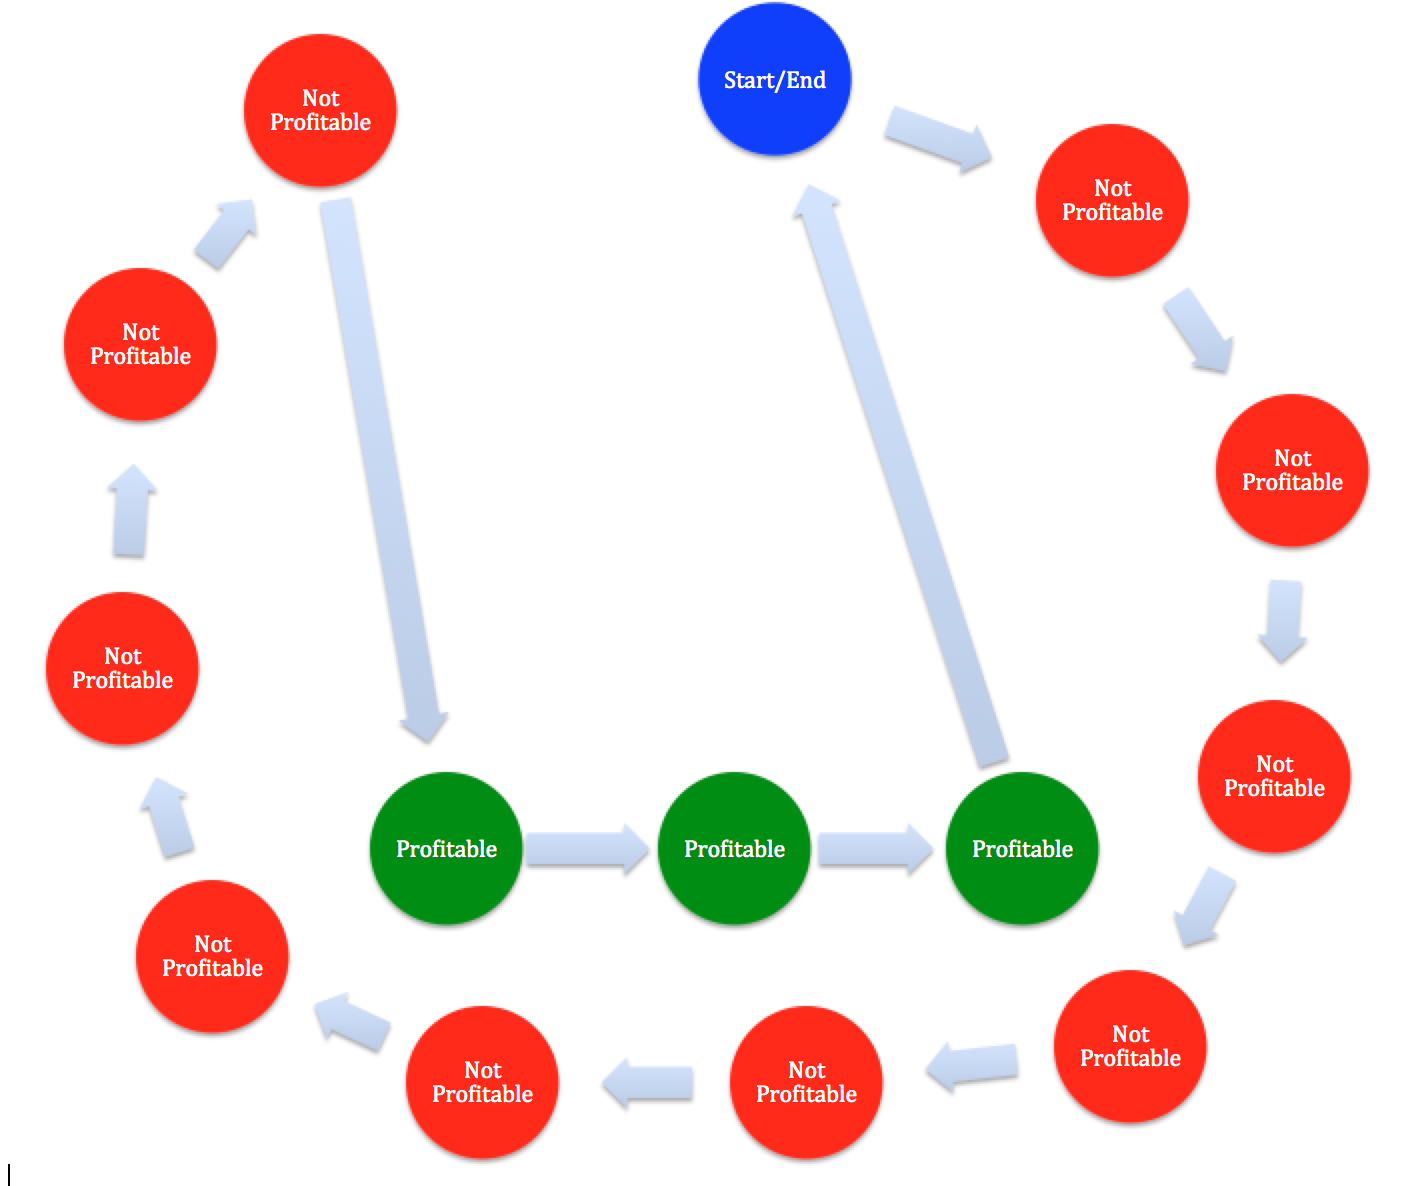
\includegraphics[width=80mm]{TheIssue.png}
\end{figure}

\end{document}
